\documentclass[12pt,a4paper]{article}
\usepackage[utf8]{inputenc}
\usepackage{geometry}
\usepackage{hyperref}
\usepackage{enumitem}
\usepackage{longtable}
\usepackage{array}
\usepackage{graphicx}
\usepackage{tikz}
\usetikzlibrary{positioning, arrows.meta}

\geometry{margin=1in}

\title{
    \vspace*{2cm}
    \Huge\textbf{Intelligent AI Interview Platform}\\
    \LARGE{Internship Project Report --- Version 3.0}\\
    \vspace{1cm}
    \large{Development, Cloud Deployment, and Final Status}
    \vspace{2cm}
}

\author{
    \textbf{Developed By:}\\
    Gagana K\\
    Rakshitha K\\
    \vspace{1cm}
    \textbf{Institution:}\\
    RV University, Bangalore\\
    \vspace{0.5cm}
    \textbf{Company:}\\
    LNA Technologies Pvt. Ltd., Bangalore\\
    \vspace{1cm}
    \textbf{Date:}\\
    April 21, 2026
}

\date{}

\begin{document}

\maketitle
\thispagestyle{empty}
\newpage

\tableofcontents
\newpage

% =========================================================
\section{Executive Summary}
% =========================================================

The Intelligent AI Interview Platform has completed full development and cloud deployment (Version 3.0) with all intended features implemented, tested, and operational in a live AWS production environment.

\textbf{Final Deployment Status:}
\begin{itemize}[leftmargin=*]
    \item Frontend deployed on AWS Amplify: \texttt{https://main.dxxxxxxxxxxx.amplifyapp.com}
    \item Backend deployed on AWS Lambda via API Gateway
    \item All features fully functional in production
    \item Cloud database: AWS DynamoDB (3 tables)
    \item Resume storage: Amazon S3
    \item Primary AI: Amazon Nova Lite v1 via AWS Bedrock Converse API
    \item Vision AI: Groq Cloud --- Llama 3.2 Vision for behavioral analysis
\end{itemize}

This report documents the complete development lifecycle across three versions, the final system architecture, all challenges encountered and resolved, and the outcomes achieved at the conclusion of the internship.

\newpage

% =========================================================
\section{Version History and Document Submissions}
% =========================================================

\begin{longtable}{|p{2cm}|p{2.5cm}|p{9cm}|}
\hline
\textbf{Version} & \textbf{Date} & \textbf{Updates} \\
\hline
1.0 & 02-02-2026 & Initial prototype: Firebase authentication, local JSON file storage, resume upload pipeline, basic interview loop using Groq Llama 3.1 for question generation \\
\hline
2.0 & 11-02-2026 & Complete interview system: FastAPI backend, full voice and webcam integration, adaptive questioning, answer evaluation, interview history dashboard, tab-switch integrity detection \\
\hline
2.1 & 01-03-2026 & Production deployment attempt: Vercel frontend and Render backend deployed; CORS integration issues identified and documented; frontend-backend connection resolved \\
\hline
3.0 & 21-04-2026 & Full AWS migration: Lambda, API Gateway, DynamoDB, S3; Amazon Nova Lite via Bedrock as primary AI; Historical Weakness RAG system; four-level adaptive engine; Groq Vision for behavioral scoring; all features live in production \\
\hline
\end{longtable}


\newpage

% =========================================================
\section{System Architecture}
% =========================================================

\subsection{Final Production Architecture}

The platform follows a three-tier serverless architecture with clear separation between the presentation layer, logic layer, and data and intelligence layer.

\begin{center}
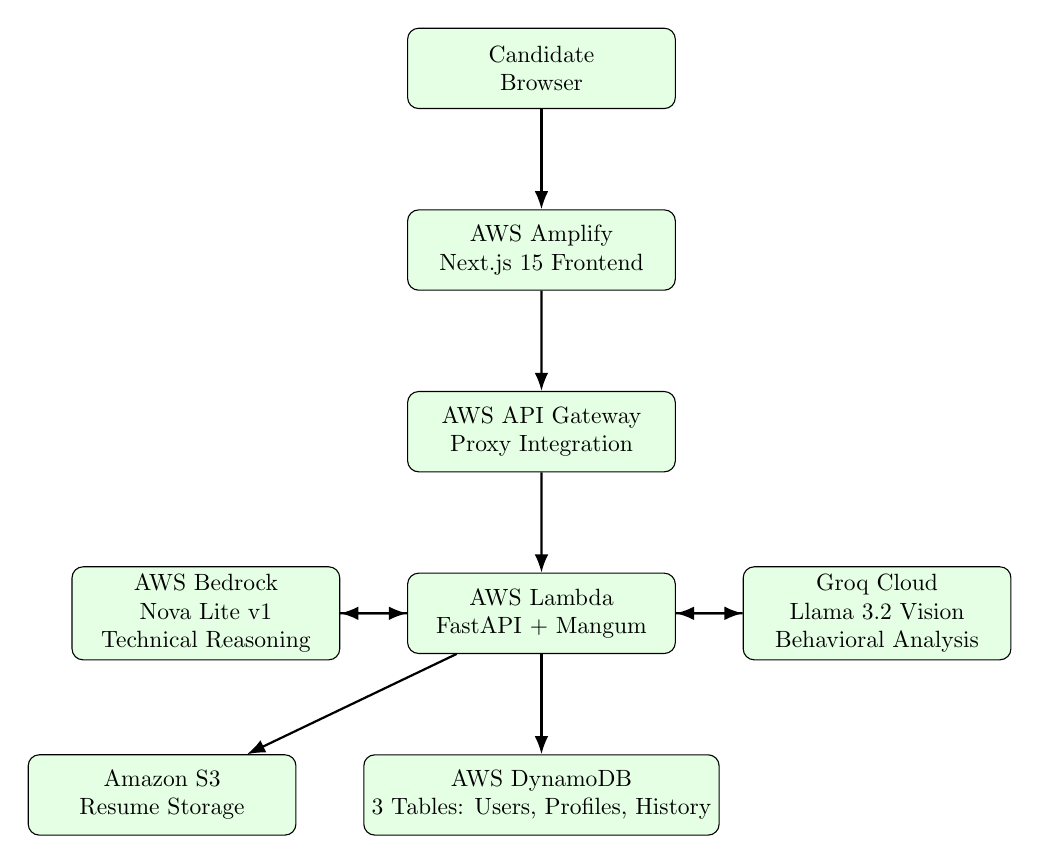
\begin{tikzpicture}[
    scale=0.85, transform shape,
    node distance=1.5cm and 1cm,
    box/.style={
        draw,
        rounded corners,
        minimum width=4cm,
        minimum height=1.2cm,
        align=center,
        fill=green!10
    },
    arrow/.style={
        -{Latex},
        thick
    }
]

\node[box] (ui) {Candidate\\Browser};
\node[box, below=of ui] (amplify) {AWS Amplify\\Next.js 15 Frontend};
\node[box, below=of amplify] (gateway) {AWS API Gateway\\Proxy Integration};
\node[box, below=of gateway] (lambda) {AWS Lambda\\FastAPI + Mangum};
\node[box, left=of lambda] (bedrock) {AWS Bedrock\\Nova Lite v1\\Technical Reasoning};
\node[box, right=of lambda] (groq) {Groq Cloud\\Llama 3.2 Vision\\Behavioral Analysis};
\node[box, below=of lambda] (db) {AWS DynamoDB\\3 Tables: Users, Profiles, History};
\node[box, left=of db] (s3) {Amazon S3\\Resume Storage};

\draw[arrow] (ui) -- (amplify);
\draw[arrow] (amplify) -- (gateway);
\draw[arrow] (gateway) -- (lambda);
\draw[arrow] (lambda) -- (bedrock);
\draw[arrow] (bedrock) -- (lambda);
\draw[arrow] (lambda) -- (groq);
\draw[arrow] (groq) -- (lambda);
\draw[arrow] (lambda) -- (db);
\draw[arrow] (lambda) -- (s3);

\end{tikzpicture}
\end{center}

\vspace{0.5cm}
\textit{Figure: Final production architecture on AWS with serverless compute, dual AI providers, and cloud persistence.}

\subsection{Component Overview}

\begin{longtable}{|p{3cm}|p{10cm}|}
\hline
\textbf{Component} & \textbf{Description} \\
\hline
Frontend & Next.js 15 application deployed on AWS Amplify. Handles user interface, interview flow, voice input via Web Speech API, and webcam capture via MediaRecorder API. \\
\hline
API Gateway & AWS API Gateway with Proxy Integration routing all HTTP requests to the Lambda function. \\
\hline
Backend & FastAPI application wrapped with Mangum and deployed on AWS Lambda. Handles resume parsing, skill extraction, adaptive interview logic, evaluation, and RAG injection. \\
\hline
Primary AI & Amazon Nova Lite v1 via AWS Bedrock Converse API. Powers skill extraction, adaptive question generation, answer evaluation, and weakness identification. \\
\hline
Vision AI & Groq Llama 3.2 Vision via Groq Cloud. Performs sub-800ms behavioral analysis from Base64 webcam frames. \\
\hline
Database & AWS DynamoDB with three tables: InterviewUsers, InterviewProfiles, and InterviewHistory. Stores user data, parsed resume skills, session history, and the growth ledger. \\
\hline
File Storage & Amazon S3 bucket storing uploaded PDF and DOCX resumes. \\
\hline
\end{longtable}

\newpage

% =========================================================
\section{Development Status}
% =========================================================

\subsection{Feature Completion Status}

\begin{longtable}{|p{6cm}|p{3cm}|p{4cm}|}
\hline
\textbf{Feature} & \textbf{Version Completed} & \textbf{Production Status} \\
\hline
User Authentication & 1.0 & Working \\
\hline
Profile Setup & 1.0 & Working \\
\hline
Resume Upload (PDF and DOCX) & 1.0 & Working \\
\hline
AI Skill Extraction & 1.0 & Working \\
\hline
Dynamic Question Generation & 2.0 & Working \\
\hline
Answer Evaluation and Scoring & 2.0 & Working \\
\hline
Voice Input (Web Speech API) & 2.0 & Working \\
\hline
Webcam Behavioral Capture & 2.0 & Working \\
\hline
Tab Switch Integrity Detection & 2.0 & Working \\
\hline
Interview History Dashboard & 2.0 & Working \\
\hline
AWS DynamoDB Persistence & 3.0 & Working \\
\hline
Amazon S3 Resume Storage & 3.0 & Working \\
\hline
AWS Lambda Deployment & 3.0 & Working \\
\hline
Nova Lite (Bedrock) Integration & 3.0 & Working \\
\hline
Groq Vision Behavioral Scoring & 3.0 & Working \\
\hline
Historical Weakness RAG System & 3.0 & Working \\
\hline
Four-Level Adaptive Engine & 3.0 & Working \\
\hline
Consolidated Single-Prompt Architecture & 3.0 & Working \\
\hline
\end{longtable}

\newpage

% =========================================================
\section{Weekly Progress Log}
% =========================================================

\begin{longtable}{|p{2cm}|p{3.5cm}|p{7cm}|}
\hline
\textbf{Week} & \textbf{Dates} & \textbf{Work Completed} \\
\hline
Week 1 & Jan 24 -- Jan 30 & Problem analysis, objective definition, development environment setup, Firebase authentication integration \\
\hline
Week 2 & Jan 31 -- Feb 6 & Authentication flow, profile setup, resume upload pipeline, initial backend API \\
\hline
Week 3 & Feb 7 -- Feb 14 & Resume parsing with pdfplumber, skill extraction prompt, question generation prototype with Groq Llama 3.1 \\
\hline
Week 4 & Feb 15 -- Feb 21 & Interview flow implementation, answer evaluation, basic scoring system \\
\hline
Week 5 & Feb 22 -- Feb 28 & Dashboard UI, interview history, score visualisation, Framer Motion animations \\
\hline
Week 6 & Mar 1 -- Mar 7 & Multimodal input pipeline: Web Speech API for voice, MediaRecorder API for webcam, Base64 frame encoding \\
\hline
Week 7 & Mar 8 -- Mar 14 & Interview Integrity System: tab detection, Alt+Tab detection, split-screen heuristic, focus polling, auto-termination \\
\hline
Week 8 & Mar 15 -- Mar 21 & AWS infrastructure setup: DynamoDB tables, S3 bucket, IAM roles, Mangum and Lambda configuration \\
\hline
Week 9 & Mar 22 -- Mar 28 & Full AWS migration for data and file storage, API Gateway configuration, CORS resolution, production deployment \\
\hline
Week 10 & Mar 29 -- Apr 4 & Amazon Nova Lite integration via Bedrock Converse API, consolidated single-prompt architecture \\
\hline
Week 11 & Apr 5 -- Apr 11 & Historical Weakness RAG system, weakness extraction logic, DynamoDB Growth Ledger \\
\hline
Week 12 & Apr 12 -- Apr 18 & Four-level adaptive engine, score clamping and validation, full end-to-end testing \\
\hline
Week 13 & Apr 19 -- Apr 21 & System load testing, bug fixes, final documentation, and project report preparation \\
\hline
\end{longtable}

\newpage

% =========================================================
\section{Challenges and Resolutions}
% =========================================================

\begin{longtable}{|p{3.5cm}|p{5cm}|p{5cm}|}
\hline
\textbf{Challenge} & \textbf{Description} & \textbf{Resolution} \\
\hline
CORS and Frontend-Backend Disconnection & After initial deployment on Vercel and Render, the frontend could not communicate with the backend due to CORS policy errors & Migrated to a unified AWS stack (Amplify and Lambda via API Gateway) which eliminated cross-origin issues entirely \\
\hline
Lambda Statelessness & FastAPI is designed for persistent servers. Lambda loses all context after each invocation & Used Mangum adapter to wrap FastAPI for Lambda. All session state is persisted to DynamoDB after every API call \\
\hline
Prompt Blowout in RAG & As candidates completed more sessions, the weakness list grew indefinitely, exceeding token limits & Implemented deduplication and a hard cap of 15 most recent weaknesses per skill \\
\hline
Video Frame Latency & Standard GPU-based cloud APIs showed 3 to 5 second delays per frame, breaking the live interview experience & Migrated video analysis to Groq LPU hardware using Llama 3.2 Vision, reducing latency to under 800 milliseconds \\
\hline
Tab Switch False Positives & API error overlays triggered window blur events causing unintended integrity penalties & Implemented an ignoreFocusLossRef guard and a 500 millisecond debounce to block cascade re-entry \\
\hline
Inconsistent AI JSON Output & Nova Lite occasionally returned malformed JSON or scores as strings such as 8/10, breaking the score parser & Added multi-strategy JSON extraction with regex fallback and score clamping between 0 and 10 \\
\hline
Groq and httpx Version Conflict & httpx 0.28 removed the proxies parameter causing incompatibility with the Groq client & Downgraded to httpx 0.27.2 in requirements.txt \\
\hline
PDF Parsing Failures & Some PDF formats caused pdfplumber extraction failures & Added pypdf as a fallback parser with graceful error handling for unreadable formats \\
\hline
\end{longtable}

\newpage

% =========================================================
\section{Results and Outcomes}
% =========================================================

\subsection{Performance Parameters}

\begin{longtable}{|p{5cm}|p{4cm}|p{4cm}|}
\hline
\textbf{Parameter} & \textbf{Target} & \textbf{Observed Result} \\
\hline
Resume Parsing Time & Less than 5 seconds & 2 to 4 seconds \\
\hline
Question Generation Latency & Less than 3 seconds & 1.5 to 2.5 seconds (Nova Lite) \\
\hline
Behavioral Frame Analysis & Real-time & Under 800 milliseconds (Groq LPU) \\
\hline
System Cold Start (Lambda) & Less than 2 seconds & 1 to 2 seconds \\
\hline
Storage Sync Latency & Real-time & Under 1 second (DynamoDB) \\
\hline
\end{longtable}

\subsection{Delivered Capabilities}

\begin{itemize}[leftmargin=*]
    \item Automated parsing of PDF and DOCX resumes with AI-driven skill extraction.
    \item Personalised interview sessions generated from the candidate's actual resume content.
    \item Four-level adaptive difficulty adjustment based on real-time answer quality assessment.
    \item Historical Weakness RAG system that retrieves and injects past technical gaps into every new session.
    \item Parallel behavioral scoring using Groq Vision AI with graceful fallback when no camera is available.
    \item Four-layer interview integrity enforcement with automatic session termination and audit logging.
    \item Persistent DynamoDB Growth Ledger tracking candidate improvement across multiple sessions.
    \item Fully serverless production deployment scaling to multiple concurrent users at near-zero idle cost.
\end{itemize}

\newpage

% =========================================================
\section{Conclusion}
% =========================================================

Over the course of thirteen weeks at LNA Technologies Pvt. Ltd., a complete Intelligent AI Interview Platform was designed, developed, and deployed from initial prototype to production-ready cloud application.

The project involved full-stack web development with Next.js and FastAPI, serverless cloud deployment on AWS Lambda and API Gateway, cloud database design with DynamoDB, large language model integration with Amazon Nova Lite via Bedrock, and real-time vision AI integration with Groq. All features defined in the initial objectives were successfully delivered and are operational in the live production environment.

The platform's primary innovation --- the Historical Weakness RAG system --- enables long-term candidate growth tracking across multiple interview sessions, a capability not present in existing academic or commercial interview automation solutions at this level of integration.

The internship provided significant practical exposure to enterprise-grade cloud architecture, generative AI integration, and production deployment practices.



\end{document}
